\section{Applications of fuzzy systems}

Fuzzy control systems are designed to regulate the behavior of other systems, often employing a PID controller where the output relies on the disparity between the desired and observed behavior. 
The general structure of a fuzzy control system is illustrated in the figure below:
\begin{figure}[H]
    \centering
    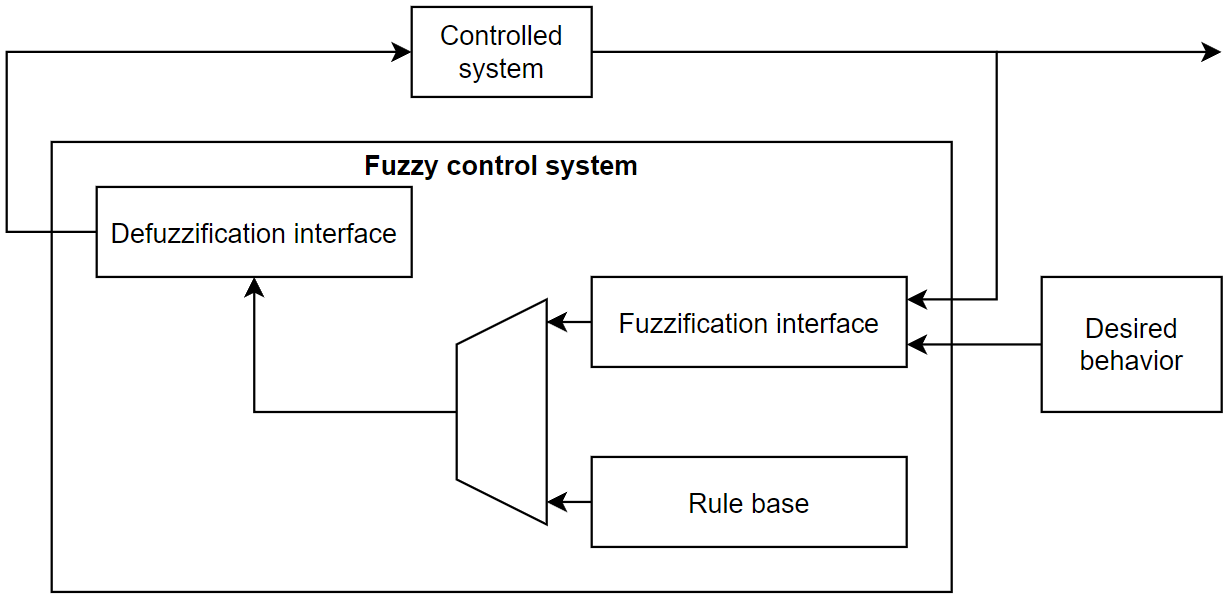
\includegraphics[width=0.5\linewidth]{images/control.png}
\end{figure}
Key attributes of a fuzzy control system include:
\begin{itemize}
    \item Robustness in the presence of noise.
    \item Control rules applicable over a broad range.
    \item Capability to model expert heuristics.
    \item Smooth action.
    \item Inherent non-linearity.
\end{itemize}
Additionally, fuzzy systems have the potential to facilitate flexible, human-like database queries. 
For instance, fuzzy sets can be employed to formulate queries such as "Provide the names of individuals who have recently made substantial investments", thereby imbuing "recently" and "a lot" with meaningful interpretations.

Fuzzy systems find applications in various domains within Artificial Intelligence, including Expert Systems, scheduling, and Decision Support Systems.